\documentclass[conference]{IEEEtran}

\usepackage{amsmath}
\usepackage{graphics}
\usepackage{graphicx}
\usepackage[english]{babel}

\bibliographystyle{/home/rsheissa/papers/midwest/IEEEtran}

\begin{document}

% paper title
\title{A CAD Tool for Automated Bandwidth Design of Negative Feedback Amplifiers}

\author{\authorblockN{Roberto Casta\~neda-Sheissa, Arturo Sarmiento-Reyes, Luis Hern\'andez-Mart\'inez and Hector V\'azquez-Leal}
\authorblockA{National Institute for Astrophysics, Optics and Electronics\\
Electronics Department, CAD Group\\
P.O. Box 51, 72000 Puebla, Pue., Mexico\\Email: rsheissa@inaoep.mx, jarocho@inaoep.mx, luish@inaoep.mx, hleal@inaoep.mx}}


% make the title area
\maketitle

\begin{abstract}
Structured design has raised as an alternative to the traditional and design approach. In the structured design, the process starts by establishing the ideal solution, which obviously fulfills a set of specifications. Hereafter, the design procedure consists in achieving a series of modifications to the ideal solution until the specs are met.

One of the key topics in the design of amplifiers is to reach a desired bandwidth (BW). This work focuses on the automation of BW design for negative feedback amplifiers through the synthesis of the nullor with active devices based on the guidelines provided by structured design.
\end{abstract}

\section{Introduction}
The design of analog amplifiers has often been considered as an art under the assumption that no systematic procedures or methodologies do exist developed so far. Experience has been the major way to produce knowledge regarding analog design. A new way to perform analog design has been developed in recent years and it has been in constant upgrade, it is called {\it structured design} \cite{verhoeven}. Herein, the main idea behind the design of negative feedback amplifiers is to divide the whole design into two main blocks, one block is the feedback network and the other block is the active part of the amplifier. As for the feedback network it is comprised of passive elements like resistors, capacitors, inducers or a combination of them.

The nullor (Figure \ref{fig:nullor}) constitutes the active (ideal) block of the amplifier. The nullor is a two-port device composed by two elements: the nullator connected at the input port and the norator connected at the output port. The transmission matrix of the nullor is composed of zeros (Eq. \ref{eq:abcd}), which indicates that the nullor possesses infinite gains for the four transfer relationships, namely voltage ($\mu$), current ($\beta$), trans-conductance ($\gamma$), and trans-impedance ($\zeta$). Since the nullor is an ideal element it is necessary to achieve its synthesis with an active device, such as BJT or MOS transistors.

\begin{equation}\label{eq:abcd}
{K}
=
\left [ \begin{array}{cc}
\frac{1}{\mu}& \frac{1}{\gamma} \\\\
\frac{1}{\zeta}& \frac{1}{\beta}
\end{array}
\right ]
=
\left [ \begin{array}{cc}
0 & 0 \\ 0 & 0
\end{array}
\right ]
\end{equation}

\begin{figure}[hbtp]
	\centering
	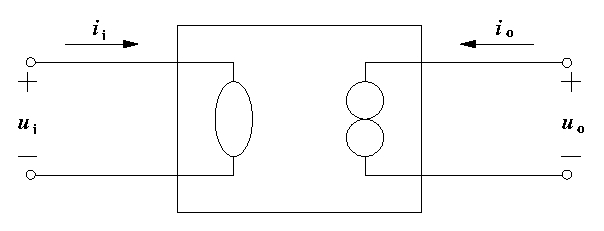
\includegraphics[scale=.7]{figures/fig_nullor.eps}
	\caption{The nullor.}
	\label{fig:nullor}
\end{figure}

The design resorts to the concept of open-loop gain-poles product \cite{verhoeven}, which is used to determine whether or not the circuit has the capability to reach the desired BW  because a flat frequency response is desired for the BW, the poles of the circuit must lie in a Butterworth distribution (Figure \ref{fig:second_butterworth}). This is done by using some well-known compensation schemes, such as pole-splitting, phantom zero, resistor broad-banding, or pole-zero cancellation. The paper presents a CAD tool that automates the BW design of negative feedback amplifiers.

\begin{figure}[hbtp]
	\centering
	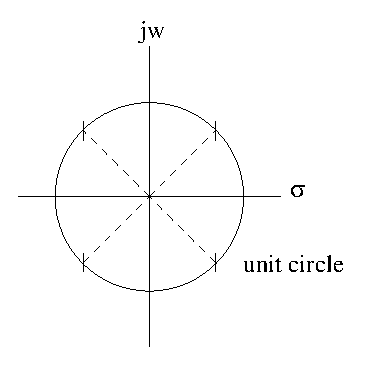
\includegraphics[scale=.7]{figures/second_ord_butterworth.eps}
	\caption{Poles of the second-order Butterworth transfer function.}
	\label{fig:second_butterworth}
\end{figure}


\section{Nullor-Based Amplifiers}
On the highest design level if a passive feedback network is connected to the nullor a basic one-loop amplifier is obtained, as seen on Figure \ref{fig:one_loop}.

\begin{figure}[hbtp]
	\centering
	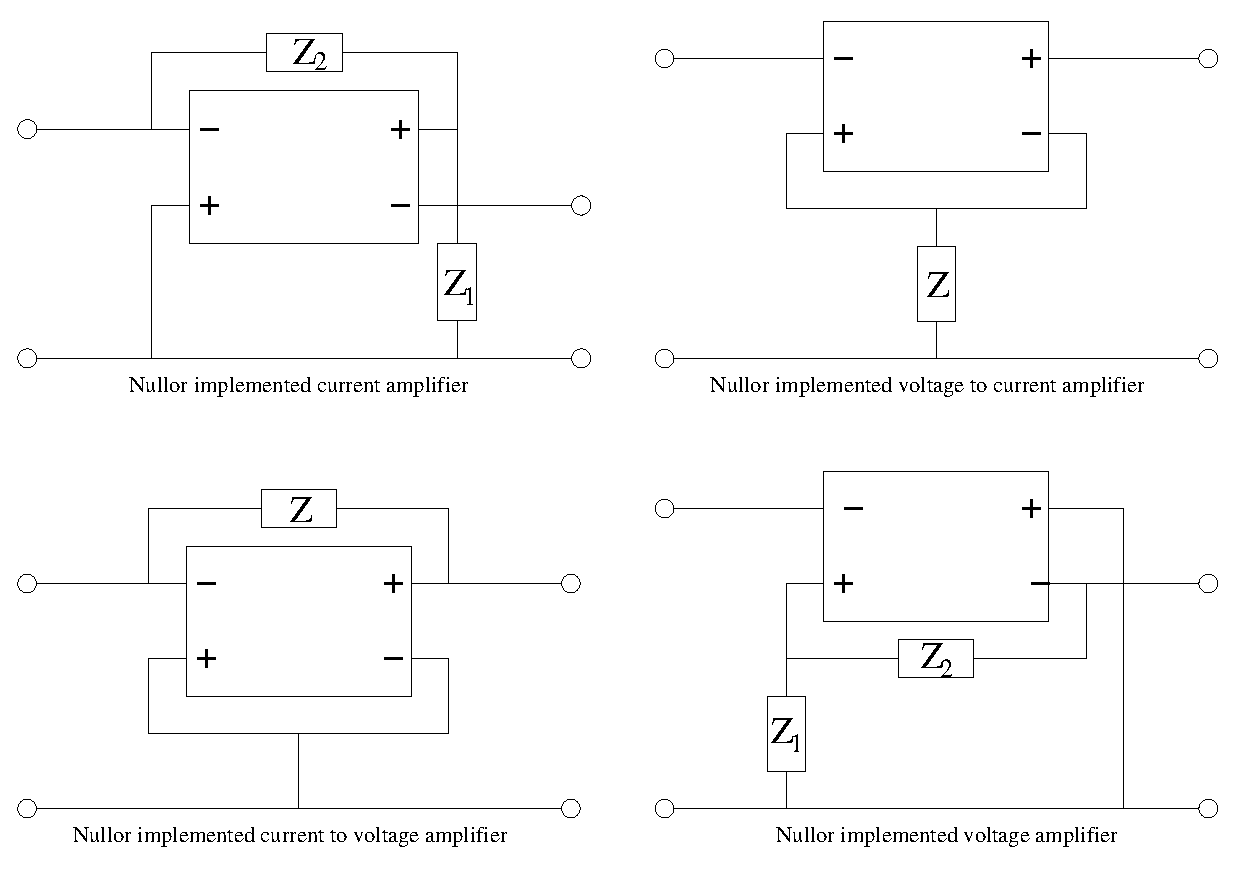
\includegraphics[scale=.4]{figures/nullor_grouped.eps}
	\caption{One-loop Negative-feedback Amplifiers.}
	\label{fig:one_loop}
\end{figure}
 
When one-loop amplifiers are combined, it is possible to generate two-loop amplifiers as shown in Figure \ref{fig:two_loop}. The combination of voltage amplifier and current amplifier are referred as the {\bf two-loop topology (A)} and the combination of transconductance and transimpedance amplifiers are denoted as the {\bf two-loop topology (B)} \cite{nordholt,stoffels}.

\begin{figure}[hbtp]
	\centering
	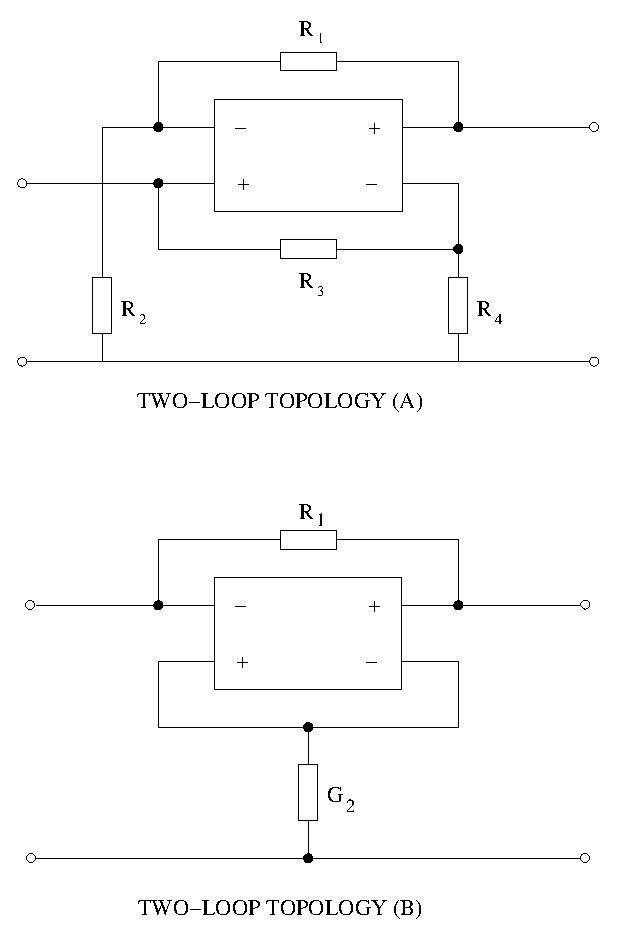
\includegraphics[scale=.5]{figures/basic_two_loops.eps}
	\caption{Two-loop Negative-feedback Amplifiers.}
	\label{fig:two_loop}
\end{figure}

Topology (B) can achieve all four kinds of transfers (voltage, current, transconductance and transimpedance), while Topology (A) can achieve all but the transconductance.

On systems design by conventional procedures designer attempts to satisfy all requirements by the judicious repeat of trial and error method. When the system is completely designed, it is verified in order to assure that complies all the function requirements, in case it fails, the design process is repeated adjusting some parameter values or modifying the configuration until all specs are accomplished \cite{ogata}.

The nullor synthesis is achieved by dividing this block into three stages to be designed:  noise, distortion and bandwidth as shown in Figure \ref{fig:block}. The noise stage is always located at the input since the noise behavior of the first stage of the active circuit is of importance. Distortion is located at the output. During these optimizations bandwidth is not taken into account. The contributions of the first and last stage to the bandwidth are taken for granted during bandwith optimization. They are taken into account, but in principle not changed.

\begin{figure}[hbtp]
	\centering
	
\includegraphics[scale=.7]{figures/blocks.eps}
	\caption{Nullor synthesis.}
	\label{fig:block}
\end{figure}

As for the bandwidth behavior it is necessary to measure the bandwidth capability of the amplifier before starting the design of this last stage. This measure can be performed in a simple way using a method called Loop-gain-Poles product (LP product). When the LP product is too low (this depends on the specified bandwidth), the design can not reach the desired bandwidth. It is assumed that an all pole Butterworth characteristic is desired \cite{chen}. When the LP product is considered large enough now the placement of the poles is of concern. This is called frequency compensation. The frequency compensation techniques are not allowed to deteriorate the former design steps, i.e. noise and distortion.

\section{Program Structure}
This program uses Maple in order to perform symbolic calculations and then substitute numerical values. The calculation process is based on the guidelines provided by \cite{wseas}. Program structure is based on the diagram in Figure \ref{fig:flow_diagram}.

\begin{figure}[hbtp]
	\centering
	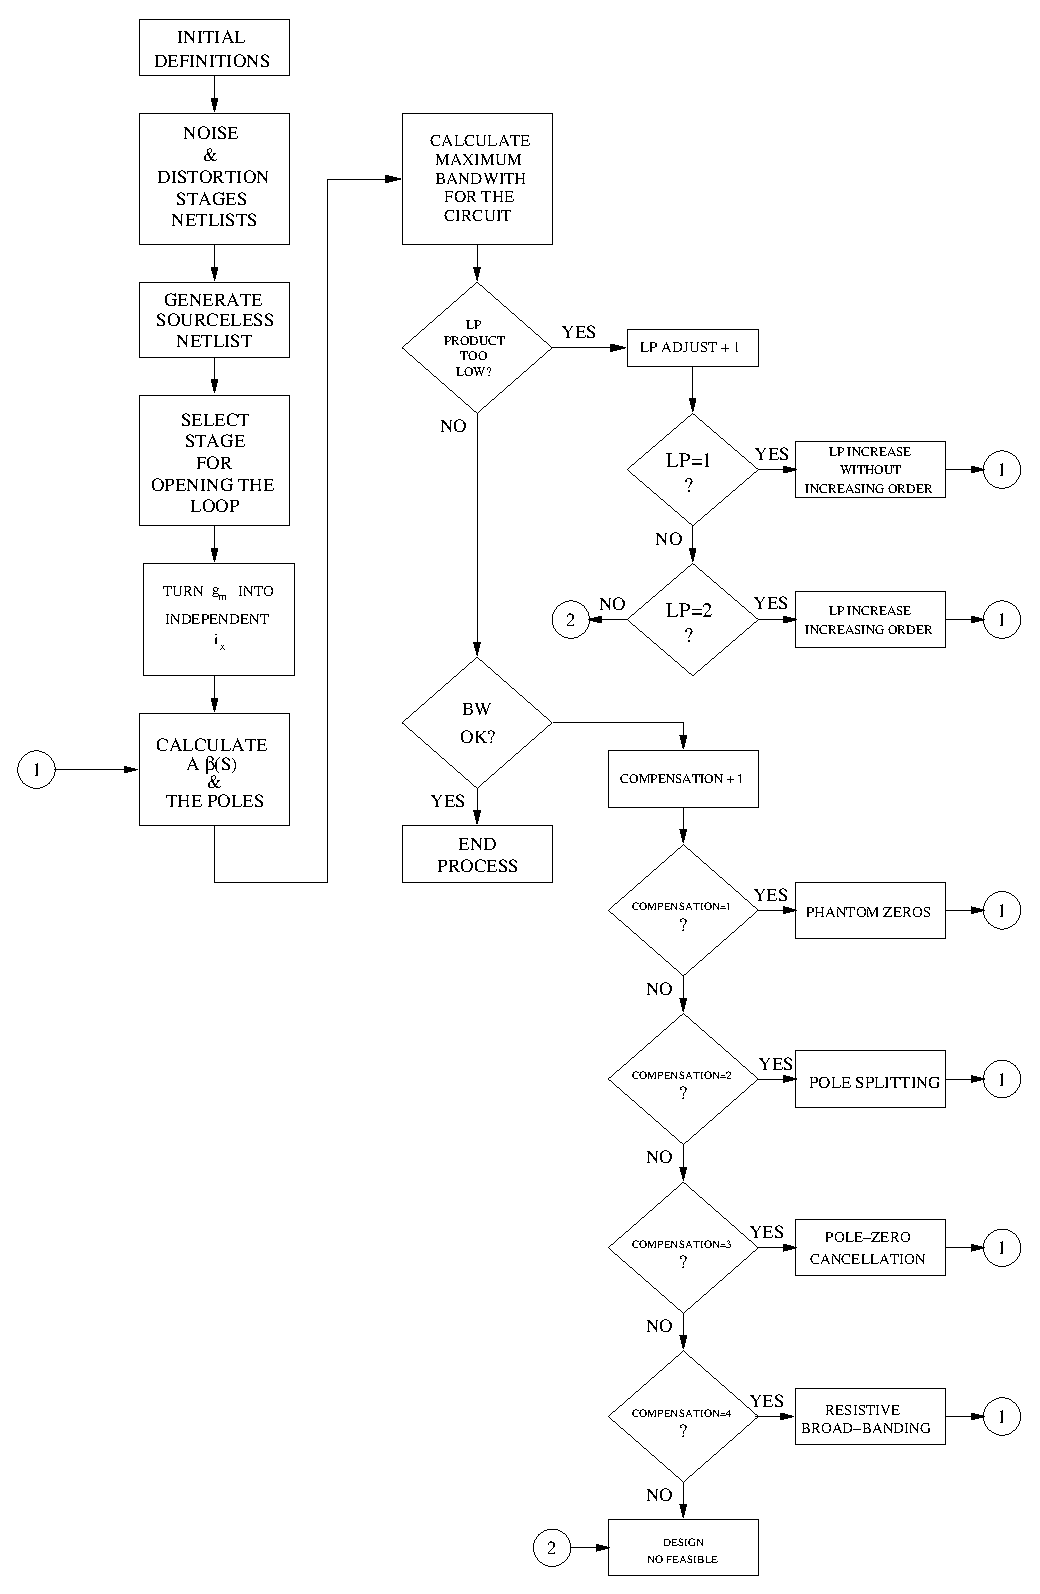
\includegraphics[scale=.5]{figures/bw_diagram.eps}
	\caption{Bandwidth Program Flow Diagram.}
	\label{fig:flow_diagram}
\end{figure}


For the active device the small signal model is employed, by this way is easier to calculate the poles and to identify where is convenient to break the loop in order to perform the open-loop gain calculation. The netlist includes the noise and distortion stages already designed and are not taken into account in any way. The first step is to calculate the transfer function as a closed-loop system, this is done by calculating the Chain-matrix for the amplifier. Next, it is necessary to find the open-loop the system gain by converting a controlled source to an uncontrolled one and making input signal equal zero, this yields the loop gain value. Once this values are found the DC-loop gain is computed as well as the poles. Using the formula \ref{eq:lp_prod} the LP product is calculated, this value indicates the maximal attainable bandwidth that circuit can achieve. If this value is too low then a routine is performed in order to increase the LP product by already found routines \cite{verhoeven}, \cite{nordholt}. 

\begin{equation}\label{eq:lp_prod}
f_{n_{max}}=\sqrt[n]{\Biggl|[1-A(0)\beta(0)]\prod_{i=1}^np_i\Biggr|}
\end{equation} 

Where $A(0)\beta(0)$ is the DC loop gain and $p_i$ are system's poles. Once the LP product adjusting routine has been performed the process is restarted from the beginning to verify that it has been increased to an acceptable value. If the maximum bandwidth computed from the LP product fulfills the bandwidth requirement provided by the user the routine is stopped and the program exits; when the maximum frequency is lower than the required bandwidth the compensation process is applied, again. After three attempts to increase the maximum frequency, if it still is achieve desired frequency then program exits indicating an error to accomplish successfully the routine. 

Granted that the circuit is capable to achieve a desired bandwidth, the next step is to design the way how the circuit is going to do it. Now the poles placement is of concern. This is called frequency compensation. Techniques for frequency compensation are not allowed to deteriorate the noise and distortion qualities already designed.

First thing to do is locate the poles position, the important ones are placed on the left side of the real axis. Poles on the right side of the real axis are not taken into account because they cannot be moved from their spot. The poles placement adjustment is performed by a routine on this order: phantom zeros, pole splitting, pole-zero cancellation and resistive broad-banding. After each compensation the LP product must be recalculated, in case that even after resistive broad-banding the design is unable to fulfill the bandwidth requirement then an error message is displayed and program exits. This mean that the design must be restructured adjusing values from the noise and distortion stages, this procedures are out of the scope of this work.

\section{Example}
The circuit under test is a transimpedance amplifier, that is, a current to voltage amplifier (Figure\ref{fig:transimp}). It is based on the exercise 9 of \cite{verhoeven}.

\begin{figure}[hbtp]
	\centering
	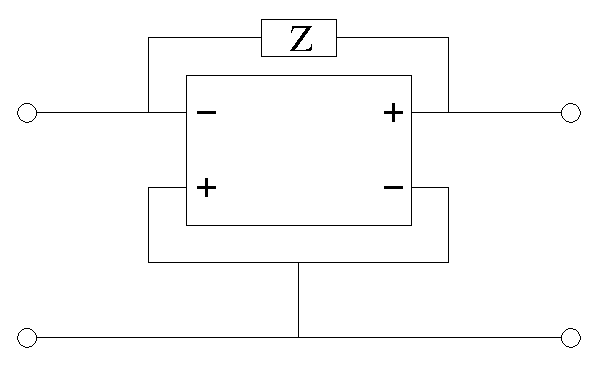
\includegraphics[scale=.5]{figures/curr_volt_amp.eps}
	\caption{Current to Voltage Amplifier.}
	\label{fig:transimp}
\end{figure}

At this point the nullor has been synthesized to fulfill the noise and distortion requirements by a single CE-stage, this has been done in order to guarantee a negative loop gain (Figure\ref{fig:transimp_1}).

\begin{figure}[hbtp]
	\centering
	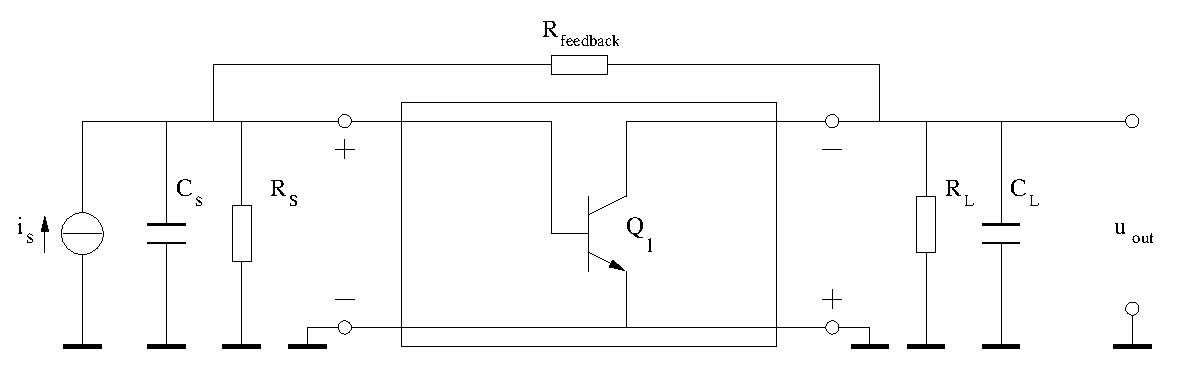
\includegraphics[scale=.45]{figures/transimp_1.eps}
	\caption{Transimpedance Amplifier with a Two-stage Nullor Implementation.}
	\label{fig:transimp_1}
\end{figure}

Using the small-signal model for the device, it turns to the scheme shown in Figure  \ref{fig:transimp_2}. The small-signal parameters for the device are:

\begin{itemize}
\item $g_m=40\text{mA/V}$
\item $c_{\pi}=4\text{pF}$
\item $r_{\pi}=2.5\text{k}\Omega$
\item $r_o=50\text{k}\Omega$
\item $\beta=100$
\end{itemize}

The values for the other components are as follows:

\begin{itemize}
\item $C_s=100\text{pF}$
\item $R_s=10\text{k}\Omega$
\item $R_{feed}=10\text{k}\Omega$
\item $R_L=10\text{k}\Omega$
\item $C_L=10\text{pF}$
\end{itemize}
 
\begin{figure}[hbtp]
	\centering
	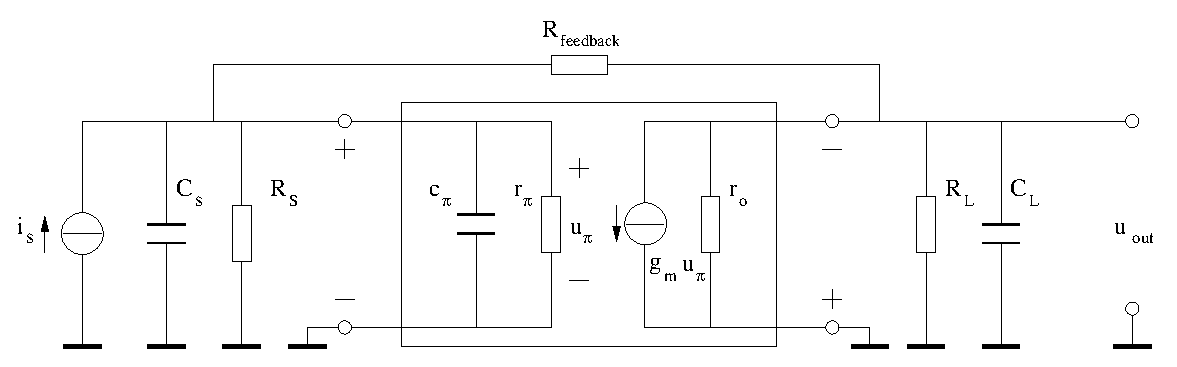
\includegraphics[scale=.45]{figures/transimp_2.eps}
	\caption{Detailed Small-signal diagram of the amplifier of Fig. \ref{fig:transimp_1}.}
	\label{fig:transimp_2}
\end{figure}

Once this values are provided for the program it calculates the LP product in order to find the maximum attainable bandwidth that this circuit can achieve. Poles are also calculated and the DC gain, as well. As stated before it is necessary to open the loop in order to perform calculations, here is easy to select the controlled source to become independent. The controlled source from the small-signal model ($g_m$) is replaced by an independent current source and transfer function is calculated. The results are:

\begin{itemize}
\item Poles - There are two located at: -827126.4896 and \mbox{-0.3592483852$\text{E}^7$} on the real axis.
\item DC loop gain - The gain is -31.78688524.
\item Maximum attainable bandwidth - If this value is low it is not possible to reach the desired bandwidth. In this case the value is $0.9718681826 \text{E}^7$.
\end{itemize}

Therefore it can be seen that the maximal bandwidth that the circuit can handle is about 9MHz and the poles can be moved, closing the loop, into the Butterworth position. This program automates the process to select the best frequency compensation method in order to obtain a Butterworth transfer function. As mentioned on the previous section there are four different types of compensation techniques. The order to be tested is as follows: phantom zero, pole-splitting, pole-zero cancellation and last resistive broad-banding. In case that program fails to obtain a satisfying value an error message appears and exits.

For the phantom zero compensation technique it is necessary to add an inductance in parallel with feedback resistor. This adds another pole to the system, this yields:

\begin{itemize}
\item Pole= -874426.1845
\item Pole= $-0.1772592078\text{E}^7+0.3071947318\text{E}^7\text{j}$
\item Pole= $-0.1772592078\text{E}^7-0.3071947318\text{E}^7\text{j}$
\item DC loop gain= -63.51612905
\item Maximum attainable bandwidth= $0.8873271607E^7$
\end{itemize}

\noindent{this technique doubles dc loop gain but reduces the maximum bandwidth and most important fact is that there is a conjugate pole. This is an undesirable behavior because poles must lay on the negative side of the real axis only. Because the failure of this compensation technique it is necessary to continue the process.}

Second compensation technique is pole-splitting. This compensation places a capacitor between $c_\pi$ and $g_m$. The main idea behind this is to split apart poles while their product remains constant such that the LP product is not changed, ideally. The values obtained are:

\begin{itemize}
\item Pole= -809142.0304
\item Pole= $-0.1751938429\text{E}^7$
\item DC loop gain= -31.78688524
\item Maximum attainable bandwidth= $0.6712677567\text{E}^7$
\end{itemize}

\noindent{here the dc loop gain is almost equal to the open loop value, nevertheless the maximum bandwidth is reduced. It is not possible to obtain a Butterworth characteristic transfer. Process continues.}

The next compensation technique is pole-zero cancellation. It is based on a compensation network to shift a pole to a lower frequency. At higher frequencies the influence of this network is removed and a zero is obtained. An additional high-frequency pole is obtained at a frequency determined by the effectiveness of the zero.Calculations yields to:

\begin{itemize}
\item Pole= $-156.3351949-.1273239544\text{E}^{-2}\text{j}$
\item Pole= $-3592990.592-.3121862787\text{E}^{-4}\text{j}$
\item Pole= $-841925.9300+.1622768058\text{E}^{-2}\text{j}$
\item DC loop gain= -31.78688524
\item Maximum attainable bandwidth= 246799.8547
\end{itemize}

\noindent{dc loop gain is within parameters but poles can not be moved to a Butterworth position. Besides the bandwidth is quite lower. Process keeps running.}

Last compensation technique is resistor broad-banding. This method acts only on one pole in contrast to the previous two methods. With a compensation network an upward shift of a single pole is realized. Values are:

\begin{itemize}
\item Pole= -3477015.922
\item Pole= -13486332.05
\item DC loop gain= -1.077621294
\item Maximum attainable bandwidth= $7108588.033\text{E}^7$
\end{itemize}

\noindent{despite the fact that the dc loop gain is the lowest from all techniques, it can achieve a large bandwidth value. It can provide a Butterworth characteristic when the loop is closed.}

By means of a simulation in hspice \cite{hspice} is verified that poles are placed at a Butterworth position. The results are:

\begin{itemize}
\item Pole= $-8.4817\text{E}^6+8.5075\text{E}^6\text{j}$
\item Pole= $-8.4817\text{E}^6-8.5075\text{E}^6\text{j}$
\end{itemize}

\noindent{calculating the angle it gives $45.09^{o}$ for a $R_{br}=122\,\Omega$. The schematic (Figure \ref{fig:transimp_3}) show where this resistor is placed.}

\begin{figure}[hbtp]
	\centering
	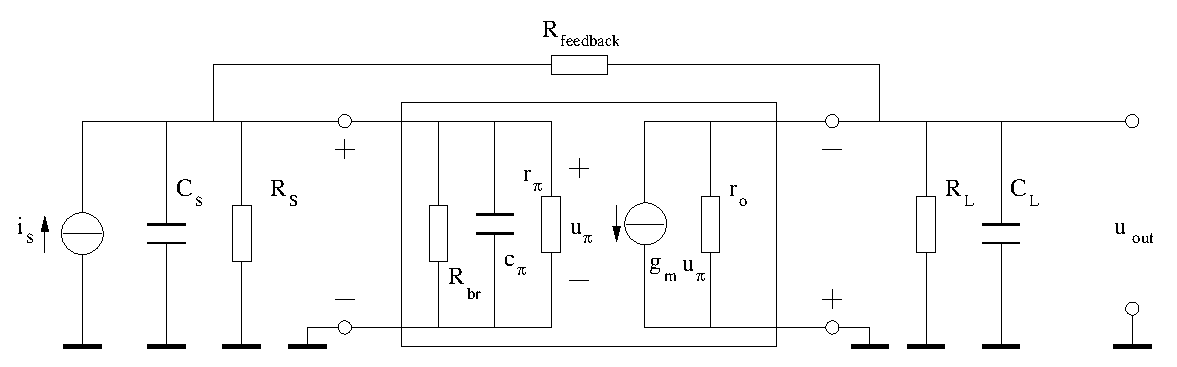
\includegraphics[scale=.45]{figures/transimp_3.eps}
	\caption{Implementation of Resistive Broad-banding.}
	\label{fig:transimp_3}
\end{figure}


\section{Conclusion}
It has been shown that by applying the theory provided by the structured design method is possible to verify if a design can accomplish the bandwith spec once the noise and distortion stages are completely designed. First by using the LP product method, designer is able to detect if the design is capable to achieve the desired bandwidth. In case LP product value is too low there are techniques to improve it. Position of the poles is another concern for the designer, a Butterworth like behavior is desired. A Maple program is capable to automate this process by providing a simple netlist, this tool performs the required calculations and provides a result. In case of failure an error message is provided to the user. 

\section*{Acknowledgment}
Roberto Casta\~neda Sheissa is holder of a scholarship from CONACyT M\'exico under contract 118652/120341. This work has been supported by a CONACyT M\'exico research project under grant 42588-Y.


\bibliography{bib/midwest}


% that's all folks
\end{document}


